\documentclass[tikz, border=5mm]{standalone}
\usetikzlibrary{shapes, arrows.meta, positioning, fit, backgrounds, calc}
\begin{document}
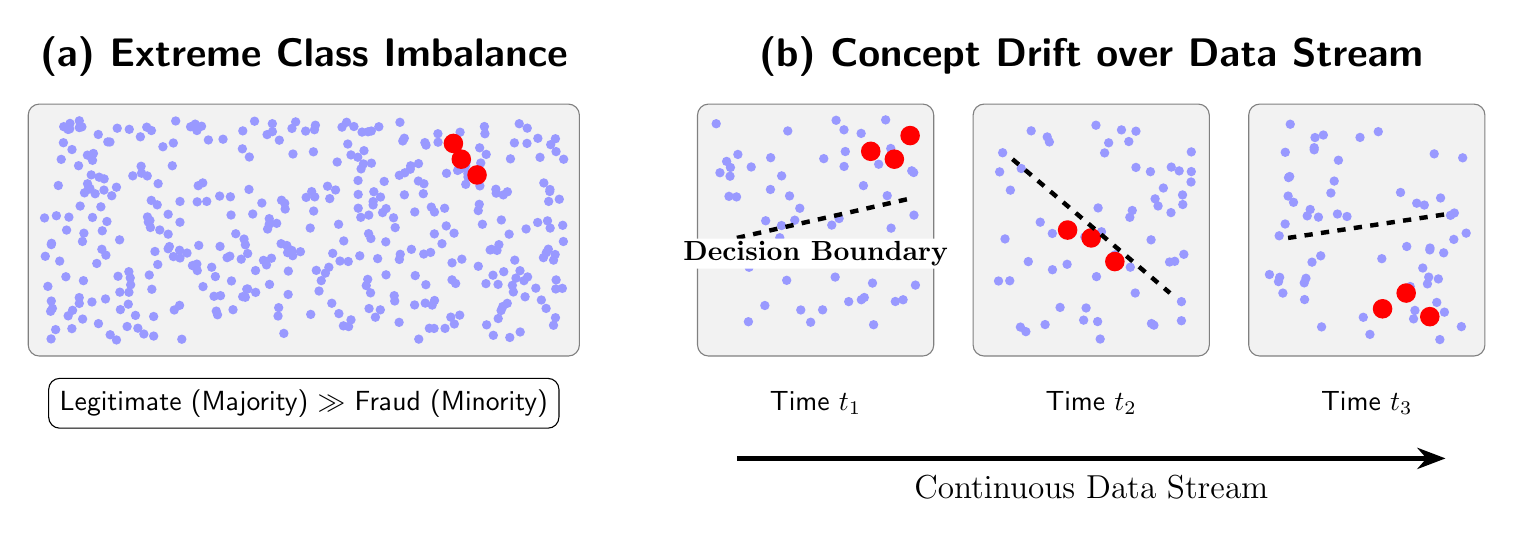
\begin{tikzpicture}[
    font=\sffamily,
    legit/.style={circle, fill=blue!40, inner sep=1.2pt},
    fraud/.style={circle, fill=red, inner sep=2.5pt},
    boundary/.style={ultra thick, dashed, draw=black}
]
\pgfmathsetseed{42}

% Panel A: Extreme Class Imbalance
\node at (0, 3.8) {\Large\textbf{(a) Extreme Class Imbalance}};
\draw[rounded corners, fill=gray!10, draw=gray] (-3.5, 0) rectangle (3.5, 3.2);

\foreach \i in {1,...,400} {
    \node[legit] at ({-3.3 + 6.6*rnd}, {0.2 + 2.8*rnd}) {};
}
% Fraud points highly localized to show imbalance
\node[fraud] at (2.0, 2.5) {};
\node[fraud] at (2.2, 2.3) {};
\node[fraud] at (1.9, 2.7) {};

\node[fill=white, draw=black, rounded corners, inner sep=4pt] at (0, -0.6) {Legitimate (Majority) $\gg$ Fraud (Minority)};

% Panel B: Concept Drift
\begin{scope}[xshift=9.5cm]
\node at (0.5, 3.8) {\Large\textbf{(b) Concept Drift over Data Stream}};

% Time t1
\node at (-3.0, -0.6) {Time $t_1$};
\draw[fill=gray!10, draw=gray, rounded corners] (-4.5, 0) rectangle (-1.5, 3.2);
\foreach \i in {1,...,60} { \node[legit] at ({-4.3 + 2.6*rnd}, {0.2 + 2.8*rnd}) {}; }
\node[fraud] at (-2.0, 2.5) {}; \node[fraud] at (-1.8, 2.8) {}; \node[fraud] at (-2.3, 2.6) {};
\draw[boundary] (-4.0, 1.5) -- (-1.8, 2.0);
\node[font=\bfseries, fill=white, inner sep=1pt, rounded corners] at (-3.0, 1.3) {Decision Boundary};

% Time t2
\node at (0.5, -0.6) {Time $t_2$};
\draw[fill=gray!10, draw=gray, rounded corners] (-1.0, 0) rectangle (2.0, 3.2);
\foreach \i in {1,...,60} { \node[legit] at ({-0.8 + 2.6*rnd}, {0.2 + 2.8*rnd}) {}; }
\node[fraud] at (0.5, 1.5) {}; \node[fraud] at (0.8, 1.2) {}; \node[fraud] at (0.2, 1.6) {};
\draw[boundary] (-0.5, 2.5) -- (1.5, 0.8);

% Time t3
\node at (4.0, -0.6) {Time $t_3$};
\draw[fill=gray!10, draw=gray, rounded corners] (2.5, 0) rectangle (5.5, 3.2);
\foreach \i in {1,...,60} { \node[legit] at ({2.7 + 2.6*rnd}, {0.2 + 2.8*rnd}) {}; }
\node[fraud] at (4.5, 0.8) {}; \node[fraud] at (4.8, 0.5) {}; \node[fraud] at (4.2, 0.6) {};
\draw[boundary] (3.0, 1.5) -- (5.0, 1.8);

% Timeline arrow
\draw[->, ultra thick, -Stealth] (-4.0, -1.3) -- (5.0, -1.3) node[midway, below=2pt, font=\large] {Continuous Data Stream};

\end{scope}

\end{tikzpicture}
\end{document}
